   \documentclass{article}
\usepackage{pgfplots}
\begin{document}
\begin{figure}
\centering

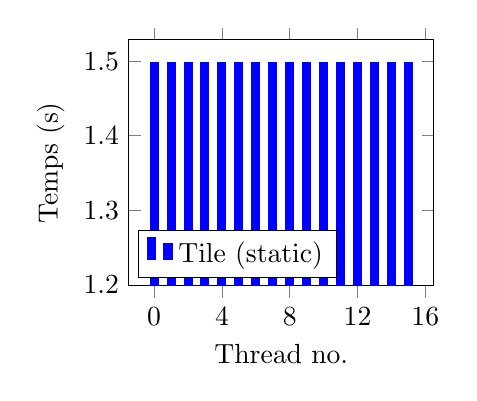
\begin{tikzpicture}
\begin{axis}[
  ybar,
  bar width=0.1cm,
  xlabel={Thread no.},
  ylabel={Temps (s)},
  ymin=1.198720,
  legend pos=south west,
  width=0.45\textwidth,
  xtick distance=4
]

% Données pour le premier graphique (à gauche)
\addplot[color=blue, fill=blue] coordinates {
  (0,1.498446) (1,1.498453) (2,1.498499) (3,1.498419) (4,1.498468) (5,1.498523) (6,1.498465) (7,1.498400) (8,1.498472) (9,1.498557) (10,1.498451) (11,1.498538) (12,1.498461) (13,1.498808) (14,1.498440) (15,1.498531)
};
\addlegendentry{Tile (static)}

\end{axis}
\end{tikzpicture}
\hfill
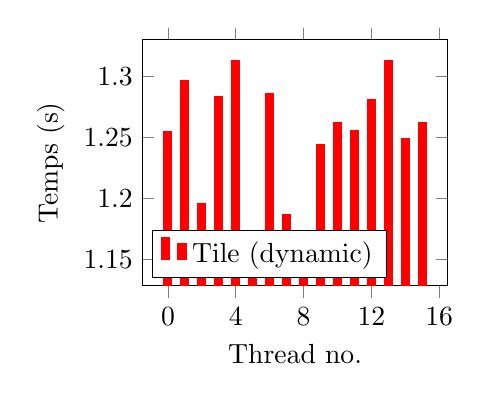
\begin{tikzpicture}
\begin{axis}[
  ybar,
  bar width=0.1cm,
  xlabel={Thread no.},
  ylabel={Temps (s)},
  ymin=,
  legend pos=south west,
  width=0.45\textwidth,
  xtick distance=4
]

% Données pour le deuxième graphique (au milieu)
\addplot[color=red, fill=red] coordinates {
  (0,1.254593) (1,1.296517) (2,1.195898) (3,1.283529) (4,1.312934) (5,1.154556) (6,1.285895) (7,1.187008) (8,1.145374) (9,1.243925) (10,1.261997) (11,1.255179) (12,1.281002) (13,1.313063) (14,1.248784) (15,1.262506)
};
\addlegendentry{Tile (dynamic)}

\end{axis}
\end{tikzpicture}
\hfill
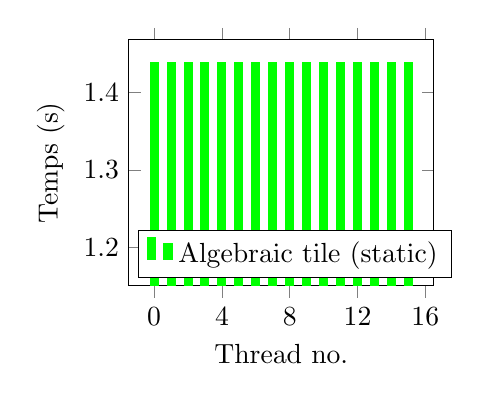
\begin{tikzpicture}
\begin{axis}[
  ybar,
  bar width=0.1cm,
  xlabel={Thread no.},
  ylabel={Temps (s)},
  ymin=1.150913,
  legend pos=south west,
  width=0.45\textwidth,
  xtick distance=4
]

% Données pour le troisième graphique (à droite)
\addplot[color=green, fill=green] coordinates {
  (0,1.438642) (1,1.438699) (2,1.438695) (3,1.438679) (4,1.438703) (5,1.438739) (6,1.438707) (7,1.438732) (8,1.438682) (9,1.438696) (10,1.438692) (11,1.438652) (12,1.438662) (13,1.438654) (14,1.438653) (15,1.438657)
};
\addlegendentry{Algebraic tile (static)}

\end{axis}
\end{tikzpicture}

\caption{Temps d'exécution des threads pour le fichier gemm.c}
\label{fig:graphes}
\end{figure}

\begin{table}[htbp]
  \centering
  \caption{Statistiques pour le fichier gemm.c}
  \begin{tabular}{|c|c|c|c|}
    \hline
    Statistique & Algebraic Tile & Tile (static) & Tile (dynamic) \\ 
    \hline
    Skewness (g1) & 0.305453 & 2.38673 & -0.76365 \\ 
    Kurtosis (g2) & -0.843138 & 5.75504 & -0.498924 \\ 
    Coefficient de variation $ \frac{\sigma}{\overline{x}} $ & 1.95551e-05 & 6.08408e-05 & 0.0404302\\ 
    Percent Imbalance metric en \% & 0.00410098 & 0.0205539 & 5.13588\\ 
    Temps d'exécution (s) &  1.438852    &  1.499104   &  1.313612   \\ 
    \hline
  \end{tabular}
\end{table}
\newpage

\begin{figure}
\centering

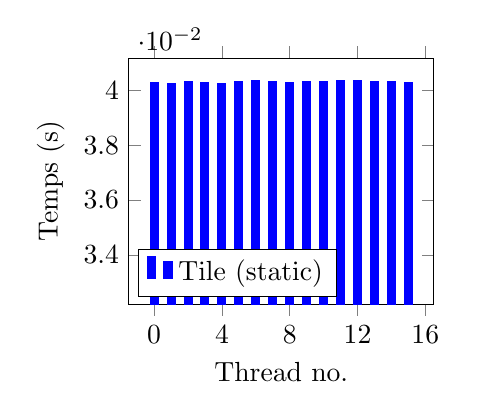
\begin{tikzpicture}
\begin{axis}[
  ybar,
  bar width=0.1cm,
  xlabel={Thread no.},
  ylabel={Temps (s)},
  ymin=.032205,
  legend pos=south west,
  width=0.45\textwidth,
  xtick distance=4
]

% Données pour le premier graphique (à gauche)
\addplot[color=blue, fill=blue] coordinates {
  (0,0.040291) (1,0.040257) (2,0.040308) (3,0.040284) (4,0.040257) (5,0.040312) (6,0.040349) (7,0.040310) (8,0.040292) (9,0.040314) (10,0.040313) (11,0.040348) (12,0.040357) (13,0.040332) (14,0.040301) (15,0.040295)
};
\addlegendentry{Tile (static)}

\end{axis}
\end{tikzpicture}
\hfill
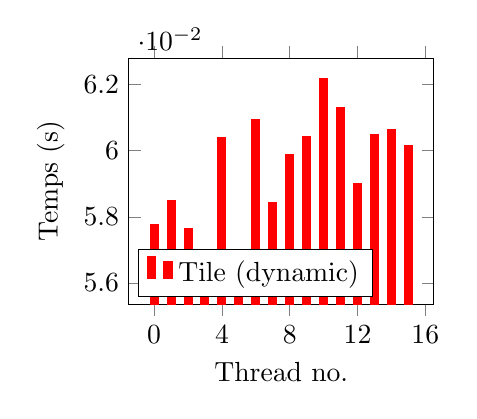
\begin{tikzpicture}
\begin{axis}[
  ybar,
  bar width=0.1cm,
  xlabel={Thread no.},
  ylabel={Temps (s)},
  ymin=,
  legend pos=south west,
  width=0.45\textwidth,
  xtick distance=4
]

% Données pour le deuxième graphique (au milieu)
\addplot[color=red, fill=red] coordinates {
  (0,0.057766) (1,0.058482) (2,0.057654) (3,0.056352) (4,0.060402) (5,0.055978) (6,0.060936) (7,0.058444) (8,0.059887) (9,0.060439) (10,0.062182) (11,0.061293) (12,0.059019) (13,0.060487) (14,0.060640) (15,0.060147)
};
\addlegendentry{Tile (dynamic)}

\end{axis}
\end{tikzpicture}
\hfill
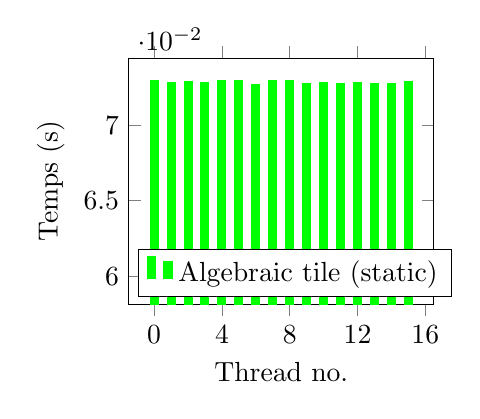
\begin{tikzpicture}
\begin{axis}[
  ybar,
  bar width=0.1cm,
  xlabel={Thread no.},
  ylabel={Temps (s)},
  ymin=.058144,
  legend pos=south west,
  width=0.45\textwidth,
  xtick distance=4
]

% Données pour le troisième graphique (à droite)
\addplot[color=green, fill=green] coordinates {
  (0,0.072941) (1,0.072794) (2,0.072865) (3,0.072793) (4,0.072961) (5,0.072962) (6,0.072680) (7,0.072939) (8,0.072947) (9,0.072757) (10,0.072830) (11,0.072789) (12,0.072857) (13,0.072740) (14,0.072766) (15,0.072882)
};
\addlegendentry{Algebraic tile (static)}

\end{axis}
\end{tikzpicture}

\caption{Temps d'exécution des threads pour le fichier gemver.c}
\label{fig:graphes}
\end{figure}

\begin{table}[htbp]
  \centering
  \caption{Statistiques pour le fichier gemver.c}
  \begin{tabular}{|c|c|c|c|}
    \hline
    Statistique & Algebraic Tile & Tile (static) & Tile (dynamic) \\ 
    \hline
    Skewness (g1) & -0.0883363 & -0.0179375 & -0.475035 \\ 
    Kurtosis (g2) & -1.14777 & -0.539625 & -0.746698 \\ 
    Coefficient de variation $ \frac{\sigma}{\overline{x}} $ & 0.00118091 & 0.000703792 & 0.0291362\\ 
    Percent Imbalance metric en \% & 0.162128 & 0.122806 & 4.71576\\ 
    Temps d'exécution (s) &  0.073368    &  0.040515   &  0.063899   \\ 
    \hline
  \end{tabular}
\end{table}
\newpage

\begin{figure}
\centering

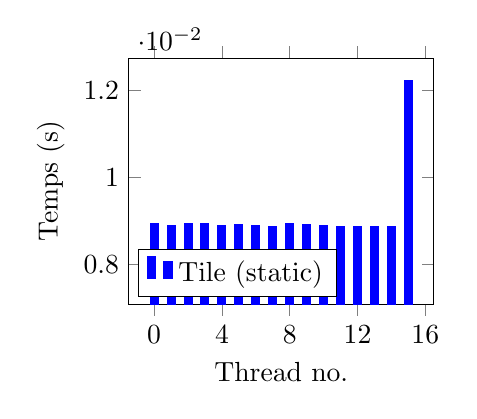
\begin{tikzpicture}
\begin{axis}[
  ybar,
  bar width=0.1cm,
  xlabel={Thread no.},
  ylabel={Temps (s)},
  ymin=.007093,
  legend pos=south west,
  width=0.45\textwidth,
  xtick distance=4
]

% Données pour le premier graphique (à gauche)
\addplot[color=blue, fill=blue] coordinates {
  (0,0.008942) (1,0.008892) (2,0.008937) (3,0.008934) (4,0.008900) (5,0.008920) (6,0.008903) (7,0.008886) (8,0.008938) (9,0.008928) (10,0.008908) (11,0.008880) (12,0.008886) (13,0.008867) (14,0.008877) (15,0.012228)
};
\addlegendentry{Tile (static)}

\end{axis}
\end{tikzpicture}
\hfill
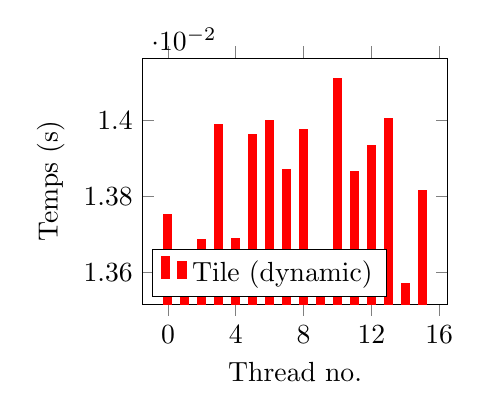
\begin{tikzpicture}
\begin{axis}[
  ybar,
  bar width=0.1cm,
  xlabel={Thread no.},
  ylabel={Temps (s)},
  ymin=,
  legend pos=south west,
  width=0.45\textwidth,
  xtick distance=4
]

% Données pour le deuxième graphique (au milieu)
\addplot[color=red, fill=red] coordinates {
  (0,0.013752) (1,0.013637) (2,0.013688) (3,0.013989) (4,0.013690) (5,0.013962) (6,0.014001) (7,0.013870) (8,0.013977) (9,0.013650) (10,0.014110) (11,0.013865) (12,0.013933) (13,0.014004) (14,0.013571) (15,0.013816)
};
\addlegendentry{Tile (dynamic)}

\end{axis}
\end{tikzpicture}
\hfill
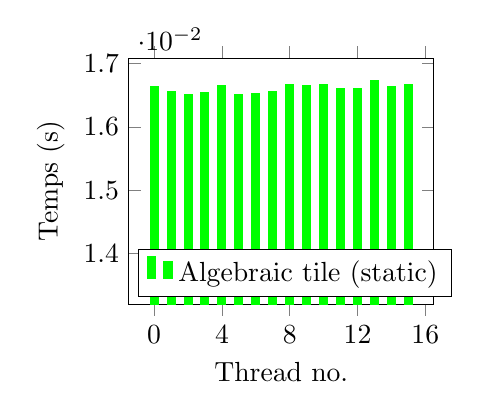
\begin{tikzpicture}
\begin{axis}[
  ybar,
  bar width=0.1cm,
  xlabel={Thread no.},
  ylabel={Temps (s)},
  ymin=.013205,
  legend pos=south west,
  width=0.45\textwidth,
  xtick distance=4
]

% Données pour le troisième graphique (à droite)
\addplot[color=green, fill=green] coordinates {
  (0,0.016639) (1,0.016561) (2,0.016507) (3,0.016541) (4,0.016652) (5,0.016508) (6,0.016526) (7,0.016555) (8,0.016675) (9,0.016658) (10,0.016673) (11,0.016601) (12,0.016599) (13,0.016732) (14,0.016641) (15,0.016675)
};
\addlegendentry{Algebraic tile (static)}

\end{axis}
\end{tikzpicture}

\caption{Temps d'exécution des threads pour le fichier gesummv.c}
\label{fig:graphes}
\end{figure}

\begin{table}[htbp]
  \centering
  \caption{Statistiques pour le fichier gesummv.c}
  \begin{tabular}{|c|c|c|c|}
    \hline
    Statistique & Algebraic Tile & Tile (static) & Tile (dynamic) \\ 
    \hline
    Skewness (g1) & -0.0582218 & 3.6095 & -0.177544 \\ 
    Kurtosis (g2) & -1.16067 & 11.043 & -1.22122 \\ 
    Coefficient de variation $ \frac{\sigma}{\overline{x}} $ & 0.00402805 & 0.0882522 & 0.0113487\\ 
    Percent Imbalance metric en \% & 0.741169 & 34.1653 & 1.91626\\ 
    Temps d'exécution (s) &  0.017008    &  0.012535   &  0.015128   \\ 
    \hline
  \end{tabular}
\end{table}
\newpage

\begin{figure}
\centering

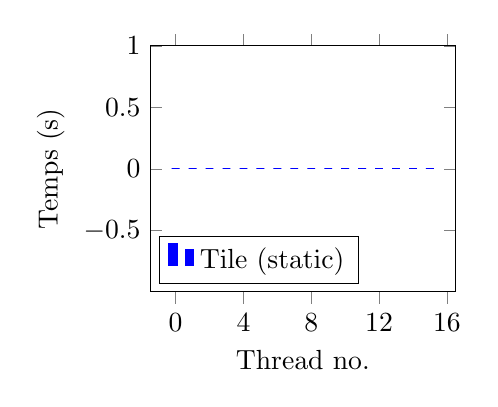
\begin{tikzpicture}
\begin{axis}[
  ybar,
  bar width=0.1cm,
  xlabel={Thread no.},
  ylabel={Temps (s)},
  ymin=0,
  legend pos=south west,
  width=0.45\textwidth,
  xtick distance=4
]

% Données pour le premier graphique (à gauche)
\addplot[color=blue, fill=blue] coordinates {
  (0,0.000000) (1,0.000000) (2,0.000000) (3,0.000000) (4,0.000000) (5,0.000000) (6,0.000000) (7,0.000000) (8,0.000000) (9,0.000000) (10,0.000000) (11,0.000000) (12,0.000000) (13,0.000000) (14,0.000000) (15,0.000000)
};
\addlegendentry{Tile (static)}

\end{axis}
\end{tikzpicture}
\hfill
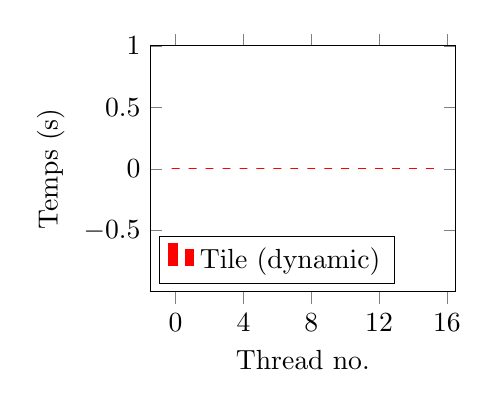
\begin{tikzpicture}
\begin{axis}[
  ybar,
  bar width=0.1cm,
  xlabel={Thread no.},
  ylabel={Temps (s)},
  ymin=,
  legend pos=south west,
  width=0.45\textwidth,
  xtick distance=4
]

% Données pour le deuxième graphique (au milieu)
\addplot[color=red, fill=red] coordinates {
  (0,0.000000) (1,0.000000) (2,0.000000) (3,0.000000) (4,0.000000) (5,0.000000) (6,0.000000) (7,0.000000) (8,0.000000) (9,0.000000) (10,0.000000) (11,0.000000) (12,0.000000) (13,0.000000) (14,0.000000) (15,0.000000)
};
\addlegendentry{Tile (dynamic)}

\end{axis}
\end{tikzpicture}
\hfill
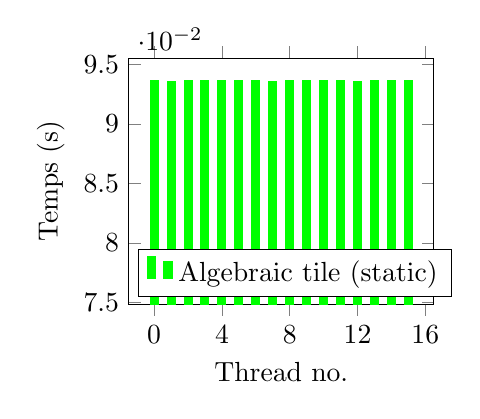
\begin{tikzpicture}
\begin{axis}[
  ybar,
  bar width=0.1cm,
  xlabel={Thread no.},
  ylabel={Temps (s)},
  ymin=.074868,
  legend pos=south west,
  width=0.45\textwidth,
  xtick distance=4
]

% Données pour le troisième graphique (à droite)
\addplot[color=green, fill=green] coordinates {
  (0,0.093627) (1,0.093591) (2,0.093627) (3,0.093652) (4,0.093645) (5,0.093647) (6,0.093647) (7,0.093600) (8,0.093637) (9,0.093636) (10,0.093617) (11,0.093637) (12,0.093585) (13,0.093618) (14,0.093645) (15,0.093636)
};
\addlegendentry{Algebraic tile (static)}

\end{axis}
\end{tikzpicture}

\caption{Temps d'exécution des threads pour le fichier symm.c}
\label{fig:graphes}
\end{figure}

\begin{table}[htbp]
  \centering
  \caption{Statistiques pour le fichier symm.c}
  \begin{tabular}{|c|c|c|c|}
    \hline
    Statistique & Algebraic Tile & Tile (static) & Tile (dynamic) \\ 
    \hline
    Skewness (g1) & -0.887797 &  &  \\ 
    Kurtosis (g2) & -0.381443 &  &  \\ 
    Coefficient de variation $ \frac{\sigma}{\overline{x}} $ & 0.00021346 &  & \\ 
    Percent Imbalance metric en \% & 0.0257402 &  & \\ 
    Temps d'exécution (s) &  1.380293    &  3.972728   &  3.678524   \\ 
    \hline
  \end{tabular}
\end{table}
\newpage

\begin{figure}
\centering

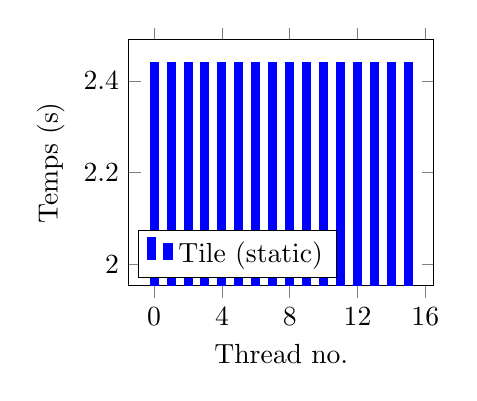
\begin{tikzpicture}
\begin{axis}[
  ybar,
  bar width=0.1cm,
  xlabel={Thread no.},
  ylabel={Temps (s)},
  ymin=1.952841,
  legend pos=south west,
  width=0.45\textwidth,
  xtick distance=4
]

% Données pour le premier graphique (à gauche)
\addplot[color=blue, fill=blue] coordinates {
  (0,2.441052) (1,2.441077) (2,2.441091) (3,2.441117) (4,2.441087) (5,2.441097) (6,2.441074) (7,2.441111) (8,2.441072) (9,2.441123) (10,2.441093) (11,2.441123) (12,2.441097) (13,2.441115) (14,2.441139) (15,2.441082)
};
\addlegendentry{Tile (static)}

\end{axis}
\end{tikzpicture}
\hfill
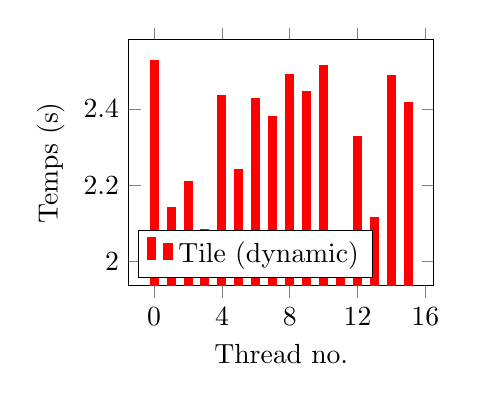
\begin{tikzpicture}
\begin{axis}[
  ybar,
  bar width=0.1cm,
  xlabel={Thread no.},
  ylabel={Temps (s)},
  ymin=,
  legend pos=south west,
  width=0.45\textwidth,
  xtick distance=4
]

% Données pour le deuxième graphique (au milieu)
\addplot[color=red, fill=red] coordinates {
  (0,2.527698) (1,2.142004) (2,2.208457) (3,2.083302) (4,2.435423) (5,2.241045) (6,2.428362) (7,2.380325) (8,2.490857) (9,2.445137) (10,2.512812) (11,1.990031) (12,2.328504) (13,2.115625) (14,2.488379) (15,2.415716)
};
\addlegendentry{Tile (dynamic)}

\end{axis}
\end{tikzpicture}
\hfill
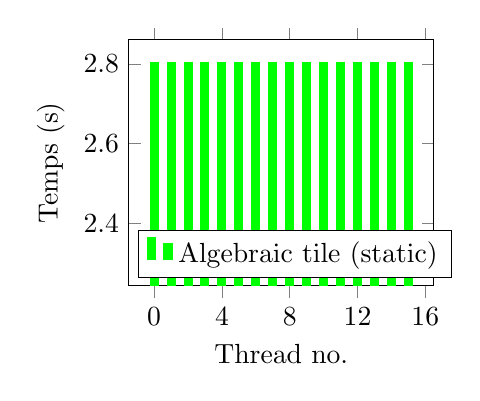
\begin{tikzpicture}
\begin{axis}[
  ybar,
  bar width=0.1cm,
  xlabel={Thread no.},
  ylabel={Temps (s)},
  ymin=2.243327,
  legend pos=south west,
  width=0.45\textwidth,
  xtick distance=4
]

% Données pour le troisième graphique (à droite)
\addplot[color=green, fill=green] coordinates {
  (0,2.804241) (1,2.804293) (2,2.804264) (3,2.804246) (4,2.804279) (5,2.804206) (6,2.804181) (7,2.804166) (8,2.804197) (9,2.804264) (10,2.804294) (11,2.804181) (12,2.804159) (13,2.804199) (14,2.804230) (15,2.804160)
};
\addlegendentry{Algebraic tile (static)}

\end{axis}
\end{tikzpicture}

\caption{Temps d'exécution des threads pour le fichier syr2k.c}
\label{fig:graphes}
\end{figure}

\begin{table}[htbp]
  \centering
  \caption{Statistiques pour le fichier syr2k.c}
  \begin{tabular}{|c|c|c|c|}
    \hline
    Statistique & Algebraic Tile & Tile (static) & Tile (dynamic) \\ 
    \hline
    Skewness (g1) & 0.130116 & -0.0154475 & -0.574694 \\ 
    Kurtosis (g2) & -1.3701 & -0.665142 & -1.03771 \\ 
    Coefficient de variation $ \frac{\sigma}{\overline{x}} $ & 1.63709e-05 & 9.15534e-06 & 0.07188\\ 
    Percent Imbalance metric en \% & 0.00263888 & 0.00159764 & 8.62009\\ 
    Temps d'exécution (s) &  2.804448 &  2.441246   &  2.538725   \\ 
    \hline
  \end{tabular}
\end{table}
\newpage

  \end{document}
